\documentclass[12pt]{article}
\usepackage{amsmath}
\usepackage{enumitem}
\usepackage{amsfonts}
\usepackage{amssymb}
\usepackage{xcolor}
\usepackage{graphicx}
\usepackage{caption}
\begin{document}
\begin{center}
\textbf\large{CHAPTER-10 \\ VECTOR ALGEBRA}
\end{center}
\section{EXERCISE - 10.2}
\begin{enumerate}
\item Compute the magnitude of the following vectors:
\begin{align*}
\vec{a}=\hat{i}+\hat{j}+k; \vec{b}=2\hat{i}-7\hat{j}-3\hat{k}; \vec{c}=\frac{1}{\sqrt{3}}\hat{i}+\frac{1}{\sqrt{3}}\hat{j}-\frac{1}{3}\hat{k}
\end{align*}
\item Write two different vectors having same magnitude.
\item Write two different vectors having same direction.
\item Find the values of x and y so that the vectors $2\hat{i}+3\hat{j}$ and $x\hat{i}+y\hat{j}$ are equal.
\item Find the scalar and vector components of the vector with initial point (2, 1) and
terminal point (– 5, 7).
\item Find the sum of the vectors $\vec{a}=\hat{i}-2\hat{j}+\hat{k}$, $\vec{b}=-2\hat{i}+4\hat{j}+5\hat{k}$ and $\vec{c}=\hat{i}-6\hat{j}-7\hat{k}$.
\item Find the unit vector in the direction of the vector $\vec{a}=\hat{i}+\hat{j}+2\hat{k}$.
\item Find the unit vector in the direction of vector $\overrightarrow{PQ}$ , where $\vec{P}$ and $\Vec{Q}$ are the points
(1, 2, 3) and (4, 5, 6), respectively.
\item For given vectors, $\vec{a}=2\hat{i}-\hat{j}+2\hat{k}$ and $\vec{b}=-\hat{i}+\hat{j}-\hat{k}$ , find the unit vector in the
direction of the vector $\vec{a}+\vec{b}$
.
\item Find a vector in the direction of vector $5\hat{i}-\hat{j}+2\hat{k}$ which has magnitude 8 units.
\item Show that the vectors $2\hat{i}-3\hat{j}+4\hat{k}$ and $-4\hat{i}+6\hat{j}-8\hat{k}$ are collinear.
\item Find the direction cosines of the vector $\hat{i}+2\hat{j}+3\hat{k}$.
\item Find the direction cosines of the vector joining the points $\Vec{A}$ (1, 2, –3) and
$\Vec{B}$(–1, –2, 1), directed from $\Vec{A}$ to $\Vec{B}$.
\item Show that the vector $\hat{i}+\hat{j}+\hat{k}$ is equally inclined to the axes OX, OY and OZ.
\item Find the position vector of a point R which divides the line joining two points $\Vec{P}$
and $\Vec{Q}$ whose position vectors are $\hat{i}+2\hat{j}-\hat{k}$ and $-\hat{i}+\hat{j}+\hat{k}$ respectively, in the
ratio 2 : 1
\begin{enumerate}[label=(\roman*)]
    \item  internally
    \item  externally
\end{enumerate}
\item Find the position vector of the mid point of the vector joining the points $\vec{P}$(2, 3, 4)
and $\vec{Q}$(4, 1, –2).
\item Show that the points A, B and C with position vectors,$\vec{a}=3\hat{i}-4\hat{j}-4\hat{k}$,$\vec{b}=2\hat{i}-\hat{j}+\hat{k}$ and $\vec{c}=\hat{i}-3\hat{j}-5\hat{k}$, respectively form the vertices of a right angled
triangle.
\item In triangle ABC (Fig 10.18), which of the following is not true:
 \begin{enumerate}
         \item $\overrightarrow{AB}+\overrightarrow{BC}+\overrightarrow{CA}$=$\vec{0}$
         \item $\overrightarrow{AB}+\overrightarrow{BC}-\overrightarrow{CA}$=$\vec{0}$
         \item $\overrightarrow{AB}+\overrightarrow{BC}-\overrightarrow{CA}$=$\vec{0}$
         \item $\overrightarrow{AB}-\overrightarrow{BC}+\overrightarrow{CA}$=$\vec{0}$
\end{enumerate}
\begin{figure}[!h]
\centering
  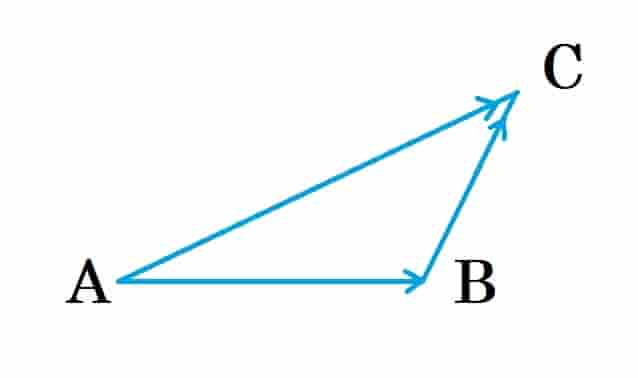
\includegraphics[width=\columnwidth]{tri.jpg}
\captionsetup{labelformat=empty}
\caption{Fig 10.18}
\label{(Fig 10.18)}
\end{figure}

\item If $\vec{a}$ and $\vec{b}$ are two collinear vectors, then which of the following are incorrect:
\begin{enumerate}
    \item $\vec{b}=\lambda\vec{a},$
 for some scalar $\lambda$
    \item $\vec{a}=\pm\vec{b}$
    \item the respective components of $\vec{a}$ and $\vec{b}$ are not proportiona
    \item both the vectors $\vec{a}$ and $\vec{b}$ have same direction, but different magnitudes.
\end{enumerate}
\end{enumerate}
\end{document}
